\begin{figure}[htbp]
  \begin{tabular}{cc}
    \begin{minipage}{0.5\hsize}
      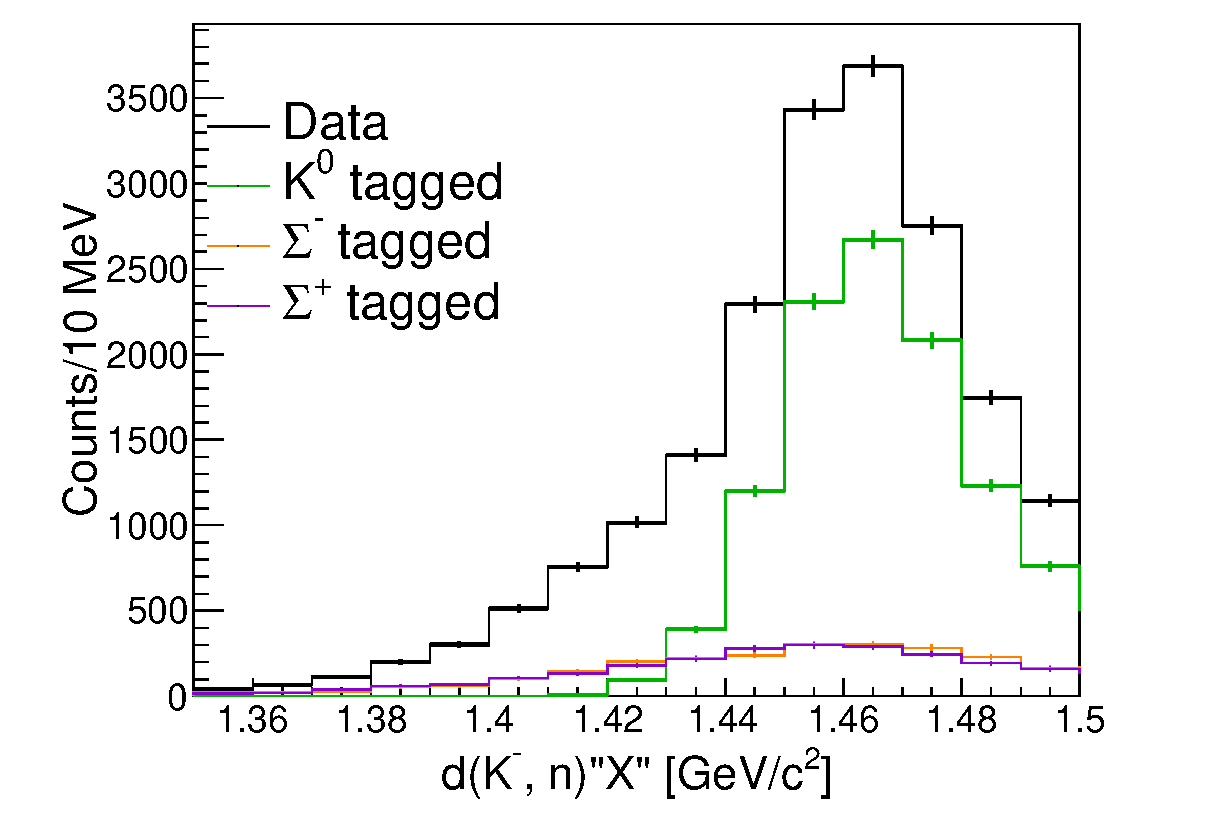
\includegraphics[width=7cm]{../pic/Run78/KN_ana_NC170_2sigma/KN_MM_all.eps}
    \end{minipage}
    \begin{minipage}{0.5\hsize}
      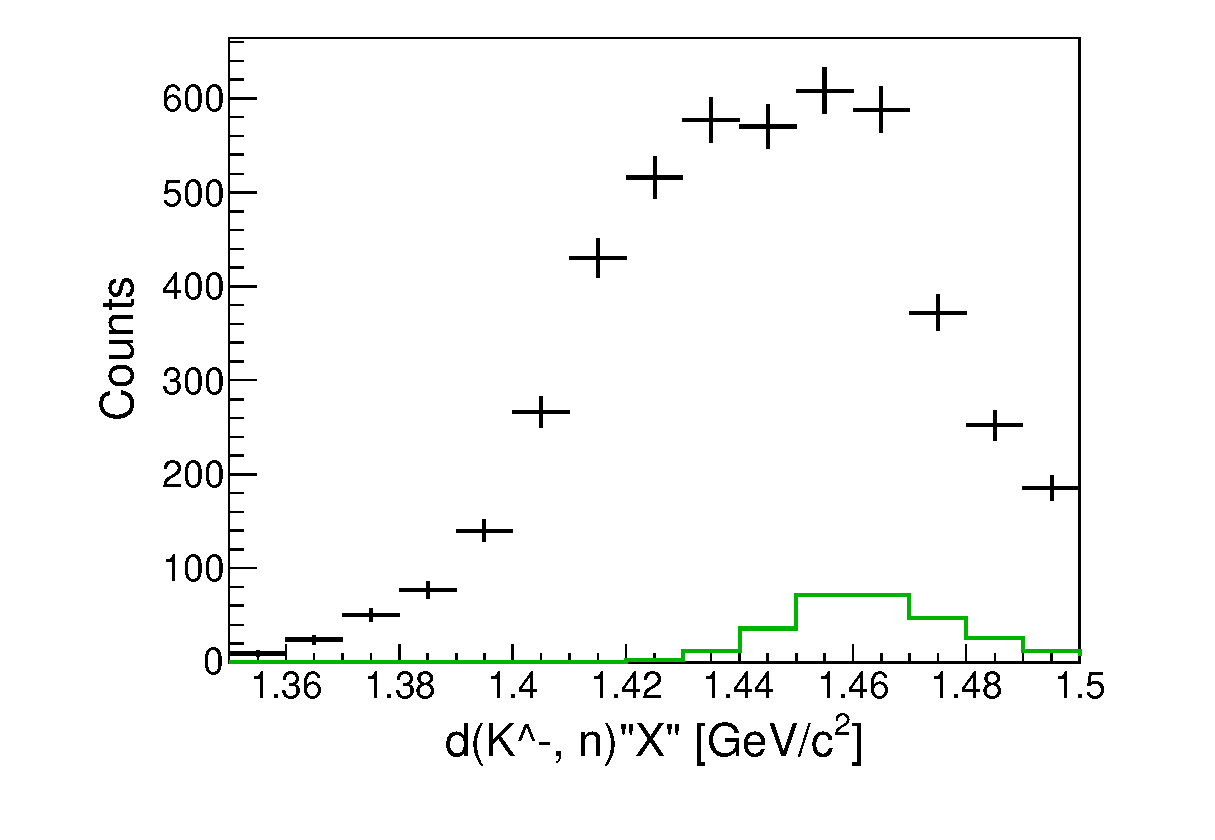
\includegraphics[width=7cm]{../pic/Dron/discussion/KN_MM_woAll.eps}
    \end{minipage}
  \end{tabular}
  \caption{    
    This figure shows the $d(K- n)$ spectrum of the $K^- d \rightarrow n \pi^+ \pi^- n$ final state.
    The left figure shows the entire event sample of $K^- d \rightarrow n \pi^+ \pi^- n$.
    The black, green, purple, and orange lines represent all events, events with identified $K^0$, $\Sigma^+$, and $\Sigma^-$, respectively.
    The right figure shows the signal events of backward-scattered $\pi\Sigma$, excluding those identified as $K^0$ or $\Sigma^+/\Sigma^-$.
%    Our signals scattered $\pi \Sigma$ backward are those other than those identified and they are represented in the right figure.
  }
  \label{fig:KN_MM_npipin}
\end{figure}
